% !TeX program = xelatex
% ============================================================
% 2007 年·普通高等学校招生考试·江苏卷 · 试题版
% 由 tools/make_editions.py 生成（重跑会覆盖本文件）；
% 题目/解析内容在 questions.tex / answers*.tex，勿在本文件内写内容。
% ============================================================
\documentclass[zihao=-4, a4paper]{ctexart}
% ============================================================
% common/preamble.tex —— 拆分版试卷项目 · 公共导言区
% 引擎：XeLaTeX；文档类 ctexart 由各版本壳文件自行声明
% 由合并书 math-gaokao-2017-2026/preamble.tex 改造而来：
%   - 页眉左右改为可重定义宏 \gkheadL / \gkheadR（各版本壳设置）
%   - hyperref 不再写死 pdftitle（壳内 \hypersetup 覆盖）
%   - 删除书籍专用的 \chaptermark 重定义与 \gkpaper 装配宏
% ============================================================

% ---------- 数学 ----------
\usepackage{amsmath}
\usepackage{amssymb}
\usepackage{mathtools}

% ---------- 绘图 ----------
\usepackage{tikz}
\usetikzlibrary{shapes.geometric, arrows.meta, calc, patterns, angles, quotes, positioning}
\usepackage{pgfplots}
\pgfplotsset{compat=1.18}

% ---------- 版面 ----------
\usepackage{geometry}
\usepackage{needspace}
\geometry{a4paper, margin=2.2cm, headheight=15pt}
% 紧凑版式（如印刷版）可在壳文件中于 \begin{document} 前再次调用 \geometry 覆盖
\usepackage{enumitem}
\setlist{itemsep=2pt, topsep=4pt, parsep=0pt}

% 中文与行内公式混排的断行弹性：
% emergencystretch 允许段落末路不通时追加伸展量；
% 降低二元/关系符罚分，允许行内长公式在 = 、+ 等处断行（否则整段外溢）
\emergencystretch=2em
\binoppenalty=700
\relpenalty=500
\usepackage{booktabs}      % 三线表
\usepackage[most]{tcolorbox}

% ---------- 选择题选项对齐 ----------
% tasks 宏包：\begin{gkopts}(列数) \task ... \end{gkopts}
% 自动等宽分栏，选项天然对齐；列数已由内容片段按选项长度写定（4/2/1）
\usepackage{tasks}
\settasks{label={}, label-width=0pt, item-indent=1.2em,
          column-sep=1em, after-item-skip=2pt, before-skip=2pt, after-skip=4pt}
\NewTasksEnvironment[style=itemize]{gkopts}[\task](4)

% ---------- 页眉页脚 ----------
\newcommand{\gkheadL}{}   % 左页眉：卷名（壳文件 \renewcommand 设置）
\newcommand{\gkheadR}{}   % 右页眉：版本名（壳文件 \renewcommand 设置）
\usepackage{fancyhdr}
\pagestyle{fancy}
\fancyhf{}
\fancyhead[L]{\small\gkheadL}
\fancyhead[R]{\small\gkheadR}
\fancyfoot[C]{\small —— 第 \thepage\ 页 ——}
\renewcommand{\headrulewidth}{0.4pt}

% ---------- 超链接（须最后加载）----------
\usepackage{hyperref}
\hypersetup{colorlinks=true, linkcolor=blue!55!black,
            bookmarksnumbered=true, unicode=true}

% ============================================================
% common/macros.tex —— 自定义命令与环境（题号、解析头、提示框等）
% 与合并书 math-gaokao-2017-2026/preamble.tex 的自定义段保持一致，
% 保证内容片段（questions.tex / answers.tex）在两个项目间可互换。
% ============================================================

% ---------- 试卷标识（壳文件 \renewcommand 设置，用于 label 命名空间）----------
\newcommand{\gkpaperid}{none}

% ---------- 题号 ----------
% 试题部分的题号：加粗编号 + 自动 \label{q:<卷id>:<题号>}
\newcommand{\gkti}[1]{\par\medskip\noindent
  \textbf{#1．}\phantomsection\label{q:\gkpaperid:#1}\ignorespaces}
% 多卷/分部重启题号时，#1 是唯一内部顺序号（交叉引用身份），#2 才是原卷显示题号。
\newcommand{\gktiwithlabel}[2]{\par\medskip\noindent
  \textbf{#2．}\phantomsection\label{q:\gkpaperid:#1}\ignorespaces}

% 解析部分的题头：小标题 + 回链到试题页
% （仅在题目与解析同文档的版本中回链有效；试题版不含解析头，无悬空引用）
\newcommand{\gksolhead}[2]{%
  \Needspace{3\baselineskip}\subsubsection*{第 #1 题\if\relax\detokenize{#2}\relax\else（#2）\fi}%
  \phantomsection\label{s:\gkpaperid:#1}%
  {\small\color{gray}（题目见第~\pageref{q:\gkpaperid:#1}~页）}\par\nopagebreak}
% 与 \gktiwithlabel 成对：显示原题号，但回链仍用唯一内部顺序号。
\newcommand{\gksolheadwithlabel}[3]{%
  \Needspace{3\baselineskip}\subsubsection*{第 #2 题\if\relax\detokenize{#3}\relax\else（#3）\fi}%
  \phantomsection\label{s:\gkpaperid:#1}%
  {\small\color{gray}（题目见第~\pageref{q:\gkpaperid:#1}~页）}\par\nopagebreak}

% ---------- 填空题空位 ----------
\newcommand{\gkblank}{\underline{\hspace{2.2em}}}

% ---------- 提示框 ----------
% 卷种提示 / 解析归属声明（醒目，浅黄）
\newtcolorbox{gknotice}{colback=yellow!8, colframe=orange!60!black,
  boxrule=0.5pt, arc=1.5pt, left=6pt, right=6pt, top=4pt, bottom=4pt,
  before skip=8pt, after skip=8pt}

% 方法提示 / 注（浅蓝，用于解析后的点评与题量说明）
\newtcolorbox{gktip}{colback=blue!4, colframe=blue!35!black,
  boxrule=0.4pt, arc=1.5pt, left=6pt, right=6pt, top=4pt, bottom=4pt,
  before skip=6pt, after skip=6pt, fontupper=\small}

% ---------- 答案行 ----------
% 解析中独立成段的"答案：X"用带底色的行呈现
\newcommand{\gkanswer}[1]{\par\smallskip\noindent
  \tcbox[width=\linewidth, tcbox width=auto limited,
         colback=green!6, colframe=green!35!black, boxrule=0.4pt,
         arc=1.5pt, left=4pt, right=4pt, top=2pt, bottom=2pt,
         nobeforeafter]{\textbf{#1}}\par\smallskip}

% ---------- 结构标题 ----------
% 结构标题后通常紧跟一个带 0.5\textheight 起始预留的解析题块；0.4 只够放标题，
% 会把下一题整体推到下一页，留下孤立的「二、填空题」等页尾标题。
\newcommand{\gkpart}[1]{\Needspace{0.6\textheight}\subsection*{#1}\nopagebreak}     % 标题 + 首题
% （一）必考题 / 解析小问标题：块式加粗段，可自动换行（\paragraph 的 run-in 版式会溢出）
\newcommand{\gksubpart}[1]{\Needspace{6\baselineskip}\par\medskip\noindent\textbf{#1}\par\nopagebreak\smallskip}

% 罗马数字Ⅰ-Ⅻ（U+2160）与圈号①②③（U+2460）划入 CJK 字符类，
% 用中文字体渲染——西文字体 Latin Modern 缺这些字形，否则整段静默丢字
\xeCJKDeclareCharClass{CJK}{"2160 -> "217F, "2460 -> "24FF}

% ============================================================
% common/questions_env.tex —— 题目 / 解析的语义包装环境
%
% questions.tex 中每道题包在 \begin{question}...\end{question} 里，
% answers.tex 中每题解析包在 \begin{answer}...\end{answer} 里；
% 题头排版仍由内容行中的 \gkti / \gksolhead 完成（见 macros.tex）。
%
% 环境本身不产生任何盒子或垂直间距（只引入一个 TeX 分组），
% 排版结果与不包裹时逐点一致。它的价值在于：
%   1. 给每道题一个机器可数的结构边界（校验脚本数环境数 = 题量）；
%   2. 为将来的条件编译留钩子——某版本可重定义环境实现按题取舍。
% ============================================================

% 环境不把整题装盒：题目与解析仍可自然跨页，但开始题块前必须为题面、
% 图形/表格或解析首段留出足够空间。仅保留 2 个 baseline 会让题干、
% 选项和图形在页边界处被拆开，形成不可打印的孤立内容；题目保留
% 0.15\textheight，在避免短题制造大段空白与避免题块拆分之间取平衡。
% 解析题块保留 0.5\textheight，以容纳“题面 + 图形/选项 + 首段解析”；
% 结构标题仍用更大的保留量；末页自然收尾由视觉复审判定。
\newenvironment{question}{\Needspace{0.15\textheight}}{}
\newenvironment{answer}{\Needspace{0.5\textheight}}{}

\renewcommand{\gkpaperid}{gk-2007-jiangsu}
\renewcommand{\gkheadL}{2007 年·普通高等学校招生考试·江苏卷 · 数学}
\renewcommand{\gkheadR}{试题版}
\hypersetup{pdftitle={2007 年·普通高等学校招生考试·江苏卷 数学 · 试题版}}
\begin{document}
\begin{center}
  {\Large\bfseries 2007 年·普通高等学校招生考试·江苏卷}\\[4pt]
  {\large 数学 · 试题版}
\end{center}
\medskip
\pdfbookmark[1]{试题}{sec:q}
% questions.tex —— 2007 年·普通高等学校招生考试·江苏卷 · 题目内容片段（无答案）
% 由 tools/generate_projects.py 依来源总账自 2007/2007_数学真题_江苏_试题.md 生成，勿手改（改源 MD 后重跑）


\gkpart{一、选择题}

\begin{question}
\gkti{1}下列函数中，周期为 $\dfrac{\pi}{2}$ 的是（　）

（A）$y=\sin\dfrac{x}{2}$

（B）$y=\sin2x$

（C）$y=\cos\dfrac{x}{4}$

（D）$y=\cos4x$

\end{question}
\begin{question}
\gkti{2}已知全集 $U=\mathbf Z$，$A=\{-1,0,1,2\}$，$B=\{x\mid x^2=x\}$，则 $A\cap\complement_UB$ 为（　）

（A）$\{-1,2\}$

（B）$\{-1,0\}$

（C）$\{0,1\}$

（D）$\{1,2\}$

\end{question}
\begin{question}
\gkti{3}在平面直角坐标系 $xOy$ 中，双曲线的中心在坐标原点，焦点在 $y$ 轴上，一条渐近线方程为 $x-2y=0$，则它的离心率为（　）

（A）$\sqrt5$

（B）$\dfrac{\sqrt5}{2}$

（C）$\sqrt3$

（D）$2$

\end{question}
\begin{question}
\gkti{4}已知两条直线 $m$，$n$，两个平面 $\alpha$，$\beta$，给出下面四个命题：

① $m\parallel n$，$m\perp\alpha\Rightarrow n\perp\alpha$；

② $\alpha\parallel\beta$，$m\subset\alpha$，$n\subset\beta\Rightarrow m\parallel n$；

③ $m\parallel n$，$m\parallel\alpha\Rightarrow n\parallel\alpha$；

④ $\alpha\parallel\beta$，$m\parallel n$，$m\perp\alpha\Rightarrow n\perp\beta$。

其中正确命题的序号是（　）

（A）①③

（B）②④

（C）①④

（D）②③

\end{question}
\begin{question}
\gkti{5}函数 $f(x)=\sin x-\sqrt3\cos x$（$x\in[-\pi,0]$）的单调递增区间是（　）

（A）$\left[-\pi,-\dfrac{5\pi}{6}\right]$

（B）$\left[-\dfrac{5\pi}{6},-\dfrac{\pi}{6}\right]$

（C）$\left[-\dfrac{\pi}{3},0\right]$

（D）$\left[-\dfrac{\pi}{6},0\right]$

\end{question}
\begin{question}
\gkti{6}设函数 $f(x)$ 定义在实数集上，它的图象关于直线 $x=1$ 对称，且当 $x\geqslant1$ 时，$f(x)=3^x-1$，则有（　）

（A）$f\left(\dfrac13\right)<f\left(\dfrac32\right)<f\left(\dfrac23\right)$

（B）$f\left(\dfrac23\right)<f\left(\dfrac32\right)<f\left(\dfrac13\right)$

（C）$f\left(\dfrac23\right)<f\left(\dfrac13\right)<f\left(\dfrac32\right)$

（D）$f\left(\dfrac32\right)<f\left(\dfrac23\right)<f\left(\dfrac13\right)$

\end{question}
\begin{question}
\gkti{7}若对于任意实数 $x$，有 $x^3=a_0+a_1(x-2)+a_2(x-2)^2+a_3(x-2)^3$，则 $a_2$ 的值为（　）

（A）$3$

（B）$6$

（C）$9$

（D）$12$

\end{question}
\begin{question}
\gkti{8}设 $f(x)=\lg\left(\dfrac{2}{1-x}+a\right)$ 是奇函数，则使 $f(x)<0$ 的 $x$ 的取值范围是（　）

（A）$(-1,0)$

（B）$(0,1)$

（C）$(-\infty,0)$

（D）$(-\infty,0)\cup(1,+\infty)$

\end{question}
\begin{question}
\gkti{9}已知二次函数 $f(x)=ax^2+bx+c$ 的导数为 $f'(x)$，$f'(0)>0$，对于任意实数 $x$ 都有 $f(x)\geqslant0$，则 $\dfrac{f(1)}{f'(0)}$ 的最小值为（　）

（A）$3$

（B）$\dfrac52$

（C）$2$

（D）$\dfrac32$

\end{question}
\begin{question}
\gkti{10}在平面直角坐标系 $xOy$ 中，已知平面区域 $A=\{(x,y)\mid x+y\leqslant1$，且 $x\geqslant0$，$y\geqslant0\}$，则平面区域 $B=\{(x+y,x-y)\mid(x,y)\in A\}$ 的面积为（　）

（A）$2$

（B）$1$

（C）$\dfrac12$

（D）$\dfrac14$

\end{question}
\gkpart{二、填空题}

\begin{question}
\gkti{11}若 $\cos(\alpha+\beta)=\dfrac15$，$\cos(\alpha-\beta)=\dfrac35$，则 $\tan\alpha\tan\beta=$\gkblank{}。

\end{question}
\begin{question}
\gkti{12}某校开设 $9$ 门课程供学生选修，其中 $A$，$B$，$C$ 三门由于上课时间相同，学校规定，每位同学选修 $4$ 门，共有\gkblank{}种不同的选修方案。（用数值作答）

\end{question}
\begin{question}
\gkti{13}已知函数 $f(x)=x^3-12x+8$ 在区间 $[-3,3]$ 上的最大值与最小值分别为 $M$，$m$，则 $M-m=$\gkblank{}。

\end{question}
\begin{question}
\gkti{14}正三棱锥 $P-ABC$ 高为 $2$，侧棱与底面 $ABC$ 成 $45^\circ$，则点 $A$ 到侧面 $PBC$ 的距离为\gkblank{}。

\end{question}
\begin{question}
\gkti{15}在平面直角坐标系 $xOy$ 中，已知 $\triangle ABC$ 顶点 $A(-4,0)$ 和 $C(4,0)$，顶点 $B$ 在椭圆 $\dfrac{x^2}{25}+\dfrac{y^2}{9}=1$ 上，则 $\dfrac{\sin A+\sin C}{\sin B}=$\gkblank{}。

\end{question}
\begin{question}
\gkti{16}某时钟的秒针端点 $A$ 到中心点 $O$ 的距离为 $5\ \mathrm{cm}$，秒针均匀地绕点 $O$ 旋转，当时间 $t=0$ 时，点 $A$ 与钟面上标 $12$ 的点 $B$ 重合，将 $A$，$B$ 两点的距离 $d$（$\mathrm{cm}$）表示成 $t$（$\mathrm{s}$）的函数，则 $d=$\gkblank{}。

\end{question}
\gkpart{三、解答题}

\begin{question}
\gkti{17}某气象站天气预报的准确率为 $80\%$，计算（结果保留到小数点后面第 $2$ 位）

（1）$5$ 次预报中恰有 $2$ 次准确的概率；

（2）$5$ 次预报中至少有 $2$ 次准确的概率；

（3）$5$ 次预报中恰有 $2$ 次准确，且其中第 $3$ 次预报准确的概率。

\Needspace{0.4\textheight}
\end{question}
\begin{question}
\gkti{18}如图，已知 $ABCD-A_1B_1C_1D_1$ 是棱长为 $3$ 的正方体，点 $E$ 在 $AA_1$ 上，点 $F$ 在 $CC_1$ 上，且 $AE=FC_1=1$。

（1）求证：$E$，$B$，$F$，$D_1$ 四点共面；

（2）若点 $G$ 在 $BC$ 上，$BG=\dfrac23$，点 $M$ 在 $BB_1$ 上，$GM\perp BF$，垂足为 $H$，求证：$EM\perp$ 面 $BCC_1B_1$；

（3）用 $\theta$ 表示截面 $EBFD_1$ 和面 $BCC_1B_1$ 所成锐二面角大小，求 $\tan\theta$。
\nopagebreak[4]
\begin{center}% 2007 年江苏卷第 18 题：棱长为 3 的正方体 ABCD-A1B1C1D1 及截面 EBFD1。
%   E 在 AA1 上（AE=1），F 在 CC1 上（FC1=1，CF=2）；
%   G 在 BC 上（BG=2/3），M 在 BB1 上，GM⊥BF 于 H。
% 来源 PDF：gaokaomath-src/普通高考/2007/2007江苏.pdf
% SHA-256：7b4d43a19a62295e52243f5c84485ce02fc6d00e98197482a09075d1c0e60bc0
% 原页：2007江苏.pdf 第 1 页（A3 三栏）第 3 栏，书页码 383。
% 重绘依据：按原页正方体斜投影、截面与 G/M/H 的位置重绘，尺寸比例按棱长 3。
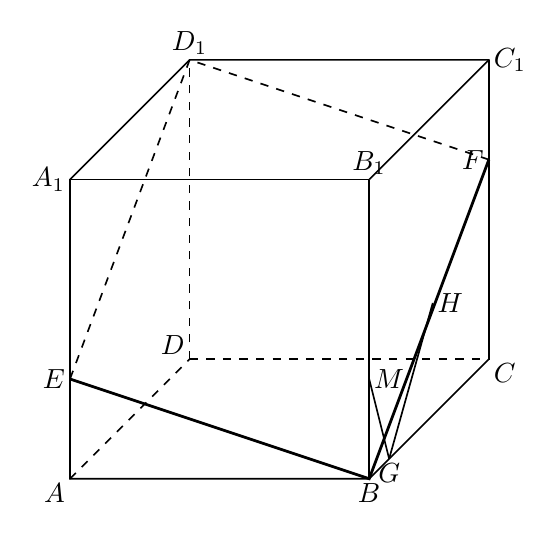
\begin{tikzpicture}[scale=0.95, semithick,
  every node/.style={inner sep=1.5pt}]

  % 正方体顶点（斜二测投影）
  \coordinate (A)  at (0,0);
  \coordinate (B)  at (4,0);
  \coordinate (C)  at (5.6,1.6);
  \coordinate (D)  at (1.6,1.6);
  \coordinate (A1) at (0,4);
  \coordinate (B1) at (4,4);
  \coordinate (C1) at (5.6,5.6);
  \coordinate (D1) at (1.6,5.6);

  % 被遮挡的棱
  \draw[dashed] (A) -- (D);
  \draw[dashed] (D) -- (C);
  \draw[dashed] (D) -- (D1);

  % 可见的棱
  \draw (A) -- (B) -- (C) -- (C1) -- (D1) -- (A1) -- cycle;
  \draw (A) -- (A1);
  \draw (B) -- (B1);
  \draw (C) -- (C1);
  \draw (B1) -- (C1);
  \draw (A1) -- (B1);

  % E、F、G、M
  \coordinate (E) at (0,1.3333);
  \coordinate (F) at (5.6,4.2667);
  \coordinate (G) at (4.2667,0.2667);
  \coordinate (M) at (4,1.3333);

  % 截面 E-B-F-D1-E
  \draw[line width=1pt] (E) -- (B) -- (F);
  \draw[dashed] (F) -- (D1);
  \draw[dashed] (D1) -- (E);

  % GM 与垂足 H（H 在 BF 上，取近似位置）
  \coordinate (H) at (4.85,2.35);
  \draw (G) -- (M);
  \draw (G) -- (H);

  % 标注
  \node[below left] at (A) {$A$};
  \node[below] at (B) {$B$};
  \node[below right] at (C) {$C$};
  \node[above left] at (D) {$D$};
  \node[left] at (A1) {$A_1$};
  \node[above] at (B1) {$B_1$};
  \node[right] at (C1) {$C_1$};
  \node[above] at (D1) {$D_1$};
  \node[left] at (E) {$E$};
  \node[left] at (F) {$F$};
  \node[below] at (G) {$G$};
  \node[right] at (M) {$M$};
  \node[right] at (H) {$H$};
\end{tikzpicture}
\end{center}
\nopagebreak[4]
\Needspace{0.4\textheight}
\end{question}
\begin{question}
\gkti{19}如图，在平面直角坐标系 $xOy$ 中，过 $y$ 轴正方向上一点 $C(0,c)$ 任作一直线，与抛物线 $y=x^2$ 相交于 $A$，$B$ 两点，一条垂直于 $x$ 轴的直线，分别与线段 $AB$ 和直线 $l$：$y=-c$ 交于 $P$，$Q$。

（1）若 $\overrightarrow{OA}\cdot\overrightarrow{OB}=2$，求 $c$ 的值；

（2）若 $P$ 为线段 $AB$ 的中点，求证：$QA$ 为此抛物线的切线；

（3）试问（2）的逆命题是否成立？说明理由。
\nopagebreak[4]
\begin{center}% 2007 年江苏卷第 19 题：抛物线 y=x^2 与过 y 轴正半轴上点 C 的直线交于 A、B，
%   过 P（AB 中点）的竖直线与 l:y=-c 交于 Q。图中按 c=2 的示意位置绘制。
% 来源 PDF：gaokaomath-src/普通高考/2007/2007江苏.pdf
% SHA-256：7b4d43a19a62295e52243f5c84485ce02fc6d00e98197482a09075d1c0e60bc0
% 原页：2007江苏.pdf 第 2 页（A3 三栏）第 1 栏，书页码 384。
% 重绘依据：按原页抛物线、直线、竖直线与 l 的相对位置重绘，c=2 仅作示意。
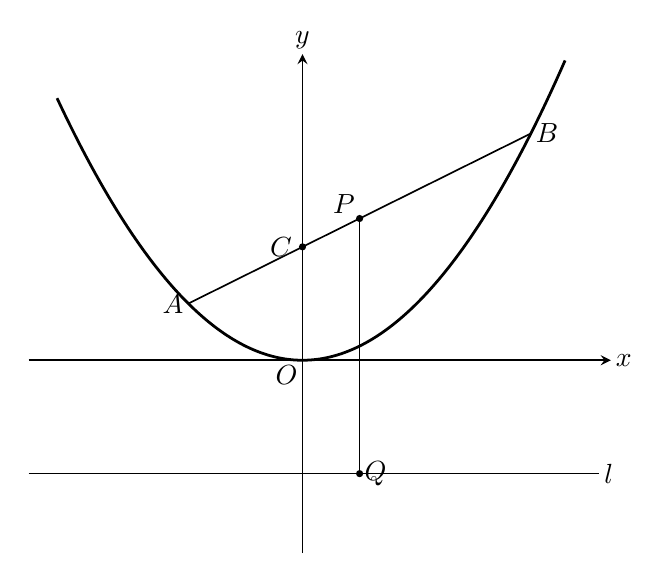
\begin{tikzpicture}[x=1.45cm, y=0.72cm, semithick,
  every node/.style={inner sep=1.5pt}]

  % 坐标轴
  \draw[->,>=stealth] (-2.4,0) -- (2.7,0) node[right] {$x$};
  \draw[->,>=stealth] (0,-3.4) -- (0,5.4) node[above] {$y$};
  \node[below left] at (0,0) {$O$};

  % 抛物线
  \draw[domain=-2.15:2.3,samples=160,line width=1pt] plot (\x,{\x*\x});

  % 直线 AB 与点
  \coordinate (C) at (0,2);
  \coordinate (A) at (-1,1);
  \coordinate (B) at (2,4);
  \coordinate (P) at (0.5,2.5);
  \coordinate (Q) at (0.5,-2);
  \coordinate (L) at (2.6,-2);

  \draw (A) -- (B);
  \draw (P) -- (Q);
  \draw (-2.4,-2) -- (L);
  \node[right] at (L) {$l$};

  \fill (C) circle (1.3pt);
  \fill (P) circle (1.3pt);
  \fill (Q) circle (1.3pt);
  \node[left=2pt] at (C) {$C$};
  \node[left] at (A) {$A$};
  \node[right] at (B) {$B$};
  \node[above left] at (P) {$P$};
  \node[right] at (Q) {$Q$};
\end{tikzpicture}
\end{center}
\nopagebreak[4]
\end{question}
\begin{question}
\gkti{20}已知 $\{a_n\}$ 是等差数列，$\{b_n\}$ 是公比为 $q$ 的等比数列，$a_1=b_1$，$a_2=b_2\neq a_1$，记 $S_n$ 为数列 $\{b_n\}$ 的前 $n$ 项和。

（1）若 $b_k=a_m$（$m$，$k$ 是大于 $2$ 的正整数），求证：$S_{k-1}=(m-1)a_1$；

（2）若 $b_3=a_i$（$i$ 是某一正整数），求证：$q$ 是整数，且数列 $\{b_n\}$ 中每一项都是数列 $\{a_n\}$ 中的项；

（3）是否存在这样的正数 $q$，使等比数列 $\{b_n\}$ 中有三项成等差数列？若存在，写出一个 $q$ 的值，并加以说明；若不存在，请说明理由。

\end{question}
\begin{question}
\gkti{21}已知 $a$，$b$，$c$，$d$ 是不全为零的实数，函数 $f(x)=bx^2+cx+d$，$g(x)=ax^3+bx^2+cx+d$。方程 $f(x)=0$ 有实数根，且 $f(x)=0$ 的实数根都是 $g(f(x))=0$ 的根；反之，$g(f(x))=0$ 的实数根都是 $f(x)=0$ 的根。

（1）求 $d$ 的值；

（2）若 $a=0$，求 $c$ 的取值范围；

（3）若 $a=1$，$f(1)=0$，求 $c$ 的取值范围。

\end{question}
\end{document}
